\section{Modellierung von Regelstrecken}{42}

\subsection{Vorgehen Modellierung von Regelstrecken}

\begin{enumerate}
    \item Einzelne Komponenten des Systems identifizieren
    \item Jede Systemkomponente als Grundglied modellieren
    \item DGL für System aufstellen (\textbf{Kräftegleichgewicht!}) \\
        \textrightarrow\ Schritt für Schritt Komponenten ineinander einsetzen \\
        \textrightarrow\ \cbl{Die interessante Grösse $y(t)$ muss ohne Vorfaktor sein!} 
    \item Aus DGL Schaltung aus Grundgliedern zeichnen \\
        \textrightarrow\ \textbf{Umformen nach höchster Ableitung}
        \textrightarrow\ Auf Output-Seite beginnen \\
        \textrightarrow\ Es braucht so viele I-Glieder wie Ordnung der DGL
\end{enumerate}


\example{Modellierung von Regelstrecke}{43}

\begin{minipage}[c]{0.45\columnwidth}
    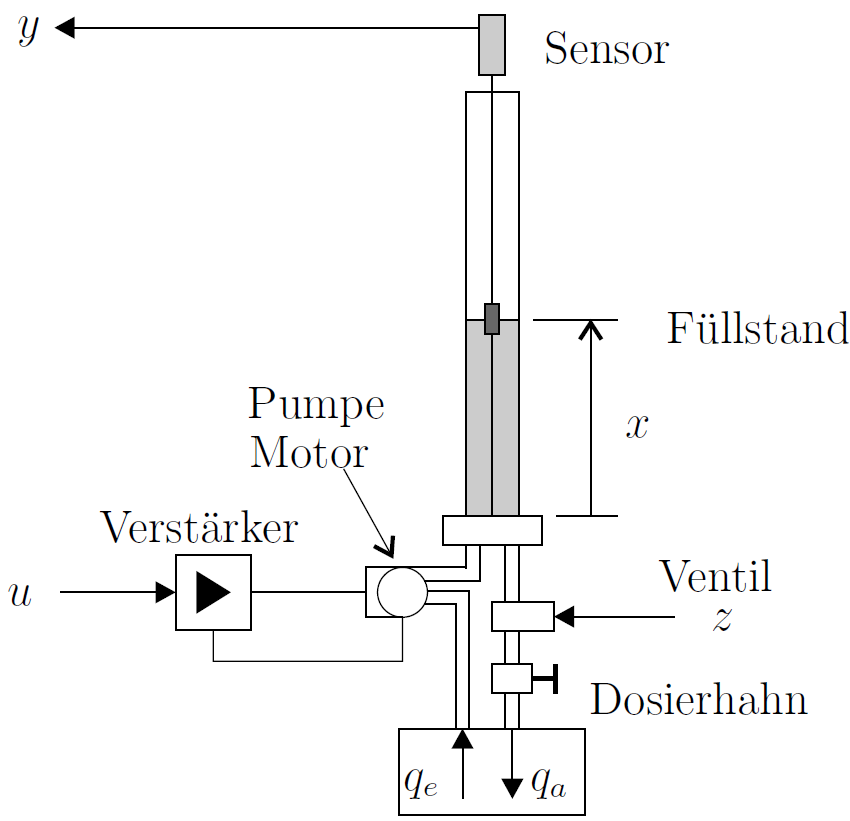
\includegraphics[width=\columnwidth]{images/modellierung_fuellprozess.png}
\end{minipage}
\hfill
\begin{minipage}[c]{0.5\columnwidth}
    \begin{enumerate}
        \setlength\itemsep{1em}

        \item \textbf{Pumpleistung $\bm{q_e}$} \\
            $q_e(t) = K_P \cdot u(t) \qquad [K_P] = \frac{\meter^3}{\volt \, \second}$

        \item \textbf{Fluss durch Ventil} \\
            \begin{minipage}[c]{0.5\columnwidth}
                $q_a(t) = \begin{cases}
                    0 & z = 0 \\
                    Q_a & z = 1 \end{cases}$
            \end{minipage}
            \hfill
            \begin{minipage}[c]{0.44\columnwidth}
                $q_a(t) = Q_a \cdot z$
            \end{minipage}

        \item \textbf{Füllstand} \\
            $\dot{x}(t) = \underbrace{ \frac{1}{A_{\phi}} }_{\substack{K_I}} (q_e(t) - q_a(t)) $

        \item \textbf{Messung $\bm{y}$} \\
            $y(t) = K_M \cdot x(t) \quad [K_M] = \frac{\volt}{\meter} $
    \end{enumerate}
\end{minipage}


\begin{minipage}[t]{0.48\columnwidth}
    \textbf{DGL aufstellen}
    \begin{align*}
        \dot{y} &= K_M \cdot \dot{x}                \\
        \dot{y} &= K_M \cdot K_I \cdot (q_e - q_a)  \\
        \dot{y} &= K_M \cdot K_I \cdot (K_P \cdot u - Q_a \cdot z)
    \end{align*}
\end{minipage}
\hfill
\begin{minipage}[t]{0.48\columnwidth}
    \textbf{Modell zeichnen} 

    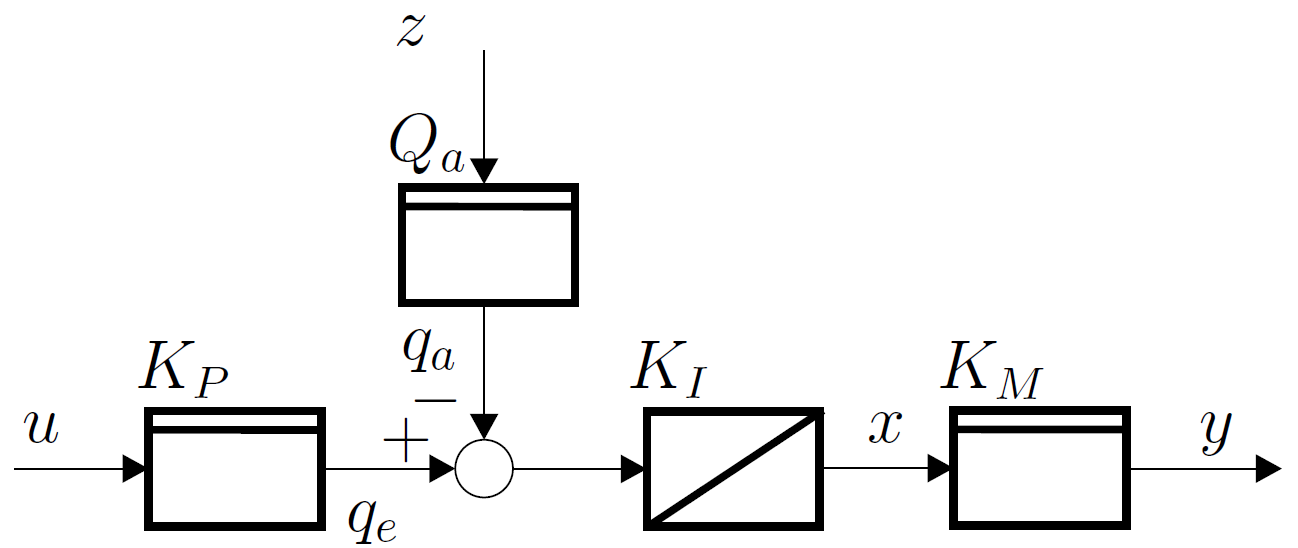
\includegraphics[width=\columnwidth]{images/modell_fuellprozess.png}
\end{minipage}


\vspace{0.2cm}

\textbf{Konstanten bestimmen} 

\begin{tabular}{ll}
    $K_M$   & Datenblatt                                                                    \\
    $K_I$   & Berechnung aus Geometrie                                                      \\
    $K_P$   & Parameter geschickt auf $0$ / bekannte Messgrössen setzen                     \\
            & $z=0, \, u(t) = A$ \quad \textrightarrow\ $\dot{y} = K_M \, K_P \, K_I \, A$  \\
    $Q_a$   & Parameter geschickt auf $0$ / bekannte Messgrössen setzen                     \\
            & $z=1, \, u(t) = 0$ \quad \textrightarrow\ $\dot{y} = - K_M \, K_I \, Q_a$
\end{tabular}


\subsubsection{Trick: Variablentransformation}

Wenn eine DGL ähnlich aussieht wie ein Grundglied (z.B. $\text{PT}_1$ oder $\text{PT}_2$), jedoch eine \textbf{Differenz von Variablen}
in der DGL vorkommt, wird die Variablentransformation angewendet.

\renewcommand{\arraystretch}{1.8}
\begin{tabular}{ll}
DGL:                                & $T \cdot \dot{y}(t) + [ \cor{y(t) - y_a(t)} ] = K \cdot u(t)$                 \\
Transformtaion:                     & $\Delta y = y - y_a \qquad \Delta \dot{y} = \dot{y} - \dot{y_a} = \dot{y}$    \\
DGL in $\text{PT}_1 \text{-Form}$:  & $T \cdot \Delta \dot{y}(t) + \cor{\Delta y(t)} = K \cdot u(t)$ 
\end{tabular}
\renewcommand{\arraystretch}{1}


\subsection{Vorgehen Blockdiagramm zu DGL}

\begin{itemize}
   \item  Anzahl Integratoren entspricht Ordnung der DGL
   \item \cbl{\textbf{Bilanz vor erstem Integrator ziehen!}}
   \item DGL umformen gemäss $\text{PT}_1$- bzw. $\text{PT}_2$-Glied
\end{itemize}

